\documentclass[letter,10pt]{article}
\usepackage{amsfonts}
\usepackage{amsmath}
\usepackage[margin=1.0in]{geometry}
\usepackage{fancyhdr}
\usepackage{hyperref}
\usepackage{multicol}
\usepackage{textcomp}
\usepackage{graphicx}
 %
\setlength{\columnsep}{0.5cm}
\pagestyle{fancy}
\fancyhf{}
\lhead{
	Live Environment Object Recognition and Model Correspondence---Project Proposal \\
	Ho, Hus, Karthikeyan, Khankin
}
\rhead{October 3rd, 2023}
\cfoot{\thepage}
\begin{document}
	\title{
		\textbf{Live Environment Object Recognition} \\\
        \textbf{and Model Correspondence} \\\
        Project Proposal
	}
	\author{
		\begin{tabular}{cccc}
			Jay Ho & Samuel Hus & Suraj Karthikeyan & David Khankin \\
			hophuc@msu.edu & hussamue@msu.edu & karthik3@msu.edu & khankind@msu.edu
		\end{tabular}
	}
	\date{October 3, 2023}
	\maketitle
	\begin{multicols}{2}
		\section{Problem Description}
            Being able to identify items in a 3D environment has been a perennial challenge in the realm of computer vision. Over the years, researchers and scientists have grappled with the complexities of transforming raw visual data into meaningful, actionable information. The nuanced interplay of algorithms, data processing techniques, and machine learning models has been meticulously explored and refined, culminating in a rich tapestry of research literature and breakthroughs. Pioneering studies have laid the groundwork for understanding the intricacies of 3D object recognition and have paved the way for the development of robust algorithms capable of deciphering the multidimensional nature of the physical world\textsuperscript{\cite{tangelder}}. 

            With this in mind, implementing the ability to have a readily available application that can help recognize items can be used on a large scale. Whether this is used in general analysis or for the purpose of maintenance, the use cases are extremely vast.
            The primary goal of this project is to take information from a live environment, such as an app that uses your phone camera, where the user is able to select objects by clicking on them, and the program will separate these objects from the background and find where this object may correspond to on an uploaded model. As a concept, this would ideally work with corresponding to a 3D model, but for the purpose of this implementation, we will remain within the constraints of corresponding to a 2D image/model. 
		\par
        \par
        The primary goal of this project is to take information from a live environment, such as an app that uses your phone camera, where the user is able to select objects by clicking on them, and the program will separate these objects from the background and find where this object may correspond to on an uploaded model. As a concept, this would ideally work with corresponding to a 3D model, but for the purpose of this implementation, we will remain within the constraints of corresponding to a 2D image/model.
        \par
        To clarify a use case instance, having uploaded a 2D solution of a puzzle, one can use the app to click on an object in the environment, and all potential areas on the puzzle image that have a potential match will be highlighted or circled. Note: This does not imply that shape will be recognized as part of this project. The goal is to match details, features, and color to a larger image and recognize if something may not be a part of that.
        \par
        Another example, we can take a look at the windows logo, where the 4 corners are red, green, blue, and yellow. If one were to select a yellow sheet of paper in the environment, the program would highlight/circle the yellow portion of the windows logo that was pre-uploaded, regardless of the shape of the paper.
        \par
        Ideally, if one were to take something with more detail, this would also be able to be recognized and properly matched to an image.
        
		\section{Related Work}
		In the realm of object extraction and segmentation, the work on BASNet stands out as a pertinent reference point for its significant contributions in this field. BASNet, an acronym for Boundary-Aware Salient Object Detection Network, has made notable strides in precisely identifying and extracting salient objects within complex environments. This technique has demonstrated a deep understanding of the spatial relationships and boundaries of objects, thereby enhancing the accuracy of object delineation. The core principle of BASNet, which emphasizes the importance of boundary information, resonates with the objectives of my research in object extraction. By leveraging the insights from BASNet's approach to extract important objects from their surroundings, our work seeks to build upon this foundation to further refine and advance the state-of-the-art in object extraction, with a particular focus on using these extracted objects in correspondence to an additional pre-processed model. In this manner, the knowledge and techniques developed in the context of BASNet provide a valuable reference and inspiration for the evolution of object extraction methodologies, contributing to the broader discourse in computer vision and image processing.\textsuperscript{\cite{basnet}}
        \par
        In recent studies within the domain of computer vision and image processing, there has been a noticeable transition in the way images are represented. Historically, images have been predominantly represented in pixel-based formats, where each pixel denotes a specific color or intensity in a fixed grid. However, the advent of graph-based representations has transformed this conventional approach. By conceptualizing images as graph structures, where nodes might represent regions or features and edges capture the relationships or proximities between these features, a more flexible and potentially richer representation is achieved.
        \par
        This paradigm shift towards graph-based representations offers a plethora of opportunities for advanced image analysis. One of the most compelling advantages is the integration of graph neural networks (GNNs) into image processing workflows. GNNs, which have demonstrated significant success in processing and analyzing structured data, can be naturally incorporated to address challenges related to image recognition when using graph-based image representations. Moreover, the inherent ability of GNNs to capture long-range dependencies and complex patterns can potentially enhance the robustness and accuracy of image recognition tasks. As the field continues to evolve, the synergy between graph-based image representations and graph neural networks promises to redefine the frontiers of image analysis and recognition techniques\textsuperscript{\cite{imagematch}}.
		
		
  
        \section{Project Milestones}
		Figure \ref{fig:milestones} below shows our project milestones and timeline to completing them. This is divided into four distinct milestones which represent key phases of our research endeavor, each with specific objectives and tasks. The following milestones are presented in chronological order: Data Compilation, Solution Development, Solution Deployment, and Iterative Enhancement.
        \par

    \begin{figure*}[t!]
        \centering
        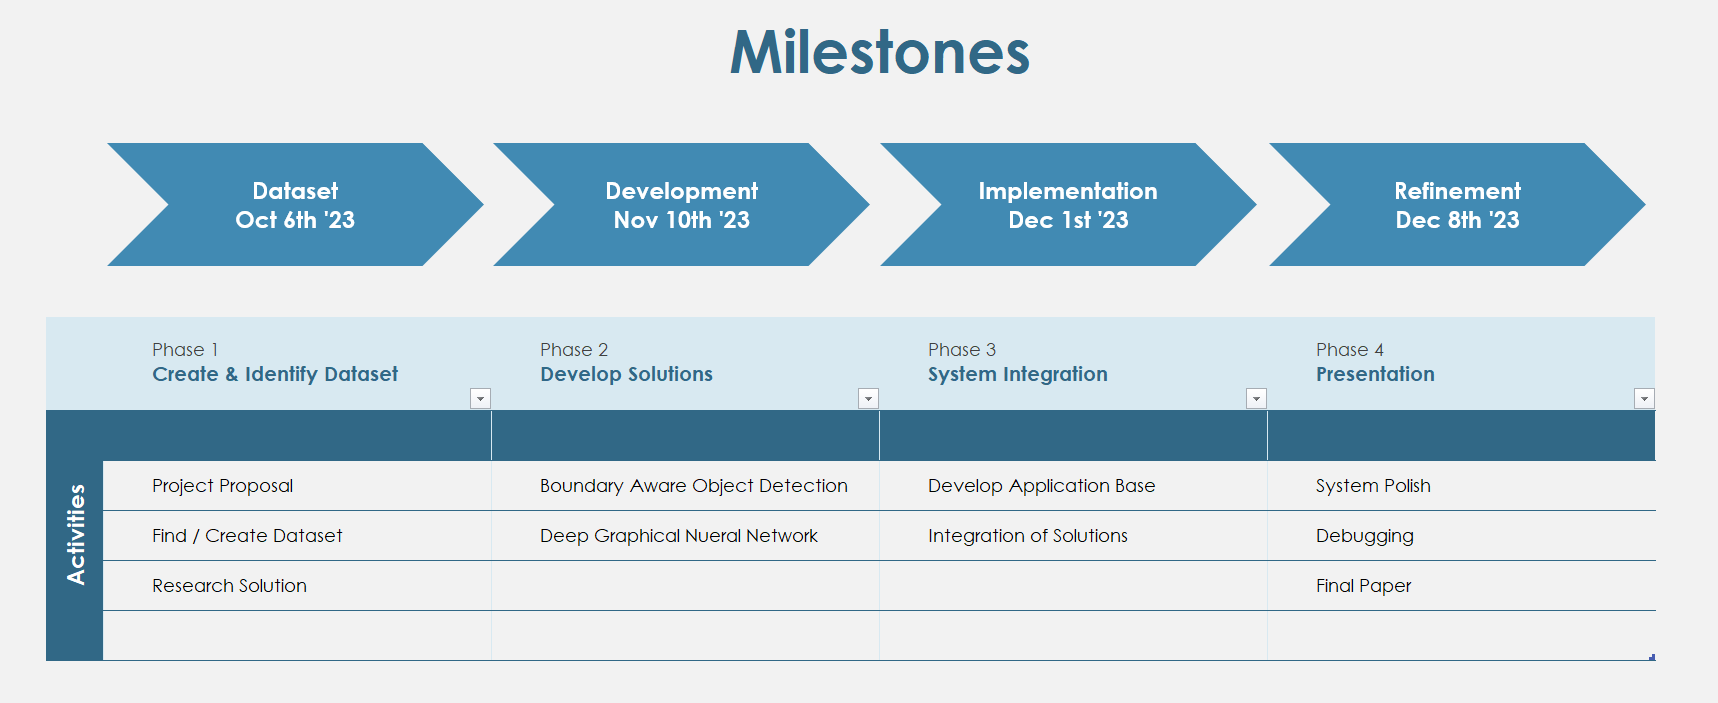
\includegraphics[width=\textwidth]{images/ProjectMilestones.png}
        \caption{Milestones and Expected Completion Dates.}
        \label{fig:milestones}
    \end{figure*}

		\begin{thebibliography}{3}
            \bibitem{tangelder}
			\textit{J. W. H. Tangelder and R. C. Veltkamp, "A survey of content based 3D shape retrieval methods," Proceedings Shape Modeling Applications, 2004 Genova, Italy, 2004, pp. 145-156, doi: 10.1109/SMI.2004.1314502.}

            \bibitem{basnet}
			\textit{X. Qin, Z. Zhang, C. Huang, C. Gao, M. Dehghan and M. Jagersand, "BASNet: Boundary-Aware Salient Object Detection," 2019 IEEE/CVF Conference on     Computer Vision and Pattern Recognition (CVPR), Long Beach, CA, USA, 2019, pp. 7471-7481, doi: 10.1109/CVPR.2019.00766..}

            \bibitem{imagematch}
                \textit{Xu, N., Nikolentzos, G., Vazirgiannis, M., Boström, H. (2022). Image Keypoint Matching Using Graph Neural Networks. In: Benito, R.M., Cherifi, C., Cherifi, H., Moro, E., Rocha, L.M., Sales-Pardo, M. (eds) Complex Networks & Their Applications X. COMPLEX NETWORKS 2021. Studies in Computational Intelligence, vol 1073. Springer, Cham.}

		\end{thebibliography}
	\end{multicols}
\end{document}

